\section{O Processador}

\label{sec:processor}

Um processador consiste em um módulo de \textit{hardware} capaz de manipular
\gls{instr-machine} armazenadas
em memória e produzir os resultados desejados através dessas instruções. Tais resultados
podem ser de cunho ou lógico-aritmético ou manipulação de dados, no geral. Tal módulo é
indispensável para o conceito de computadores como conhecemos hoje, de tal forma que, se
não fosse pela necessidade de memória para a armazenagem de dados, um processador poderia
ser a definição de um computador. Um exemplo de processador pode ser visualizado nas Figuras
\ref{subfig:processor-example-1} e \ref{subfig:processor-example-2}.

\begin{figure}[H]
    \centering
    \begin{subfigure}{.5\textwidth}
        \centering
        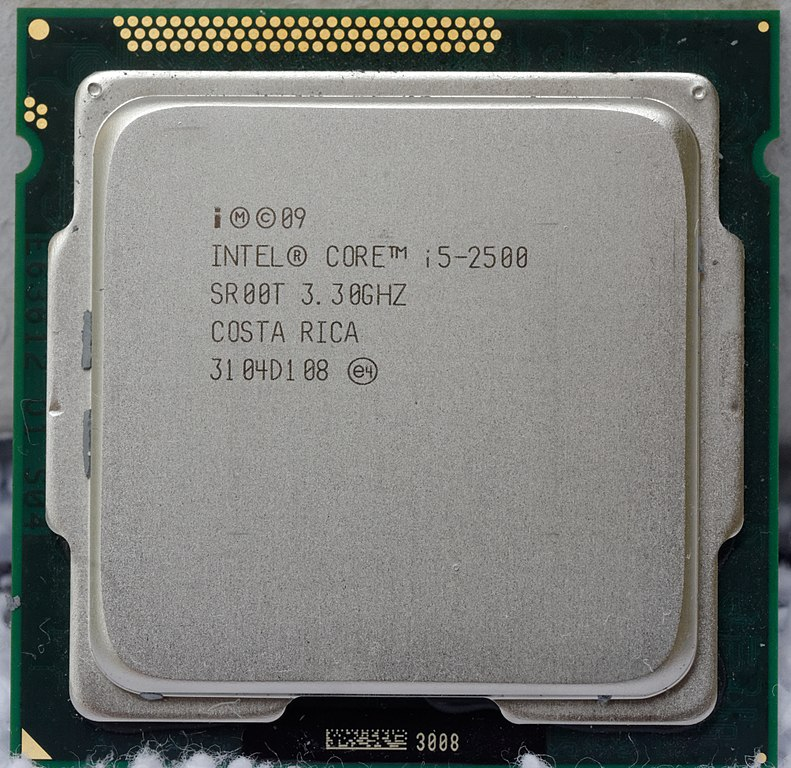
\includegraphics[width=.7\linewidth]{chapters/chp3/images/intel-i5-2500-processor.jpg}
        \caption{Um processador Intel\textsuperscript{\textregistered} 2500 \cite{wiki:i5_2500}.}
        \label{subfig:processor-example-1}
    \end{subfigure}
    \begin{subfigure}{.5\textwidth}
        \centering
        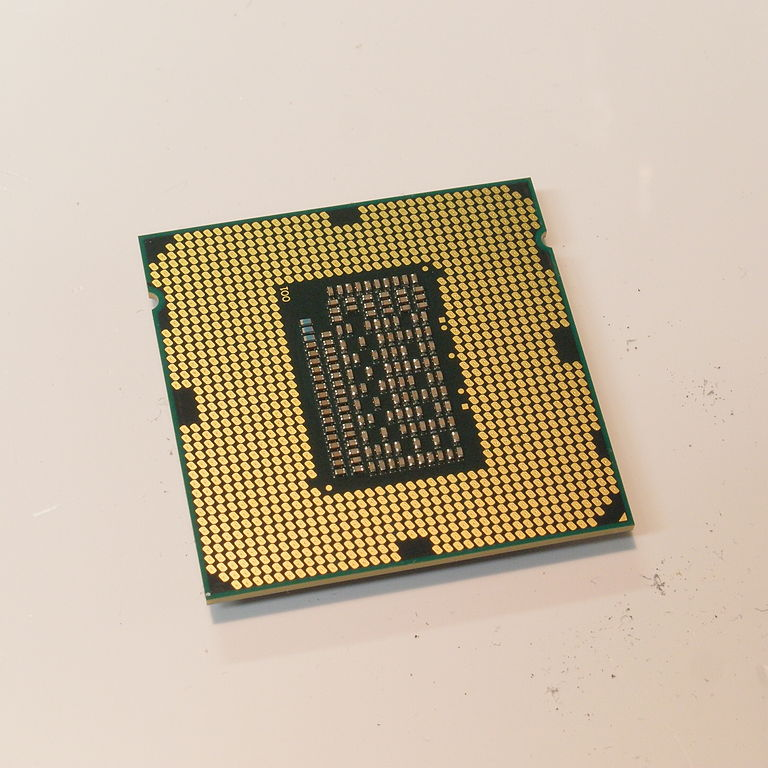
\includegraphics[width=.7\linewidth]{chapters/chp3/images/intel-i7-2600k-processor-pins.jpg}
        \caption{Os pinos de um processador Intel\textsuperscript{\textregistered} 2600 \cite{wiki:i7_2600}}
        \label{subfig:processor-example-2}
    \end{subfigure}
    \caption{Exemplos de processadores}
    \label{fig:processors}
\end{figure}